\documentclass[UTF8,a4paper,10pt]{ctexart}
\usepackage[left=3.17cm, right=3.17cm, top=2.74cm, bottom=2.74cm]{geometry}
\usepackage{amsmath}
\usepackage{graphicx,subfig}
\usepackage{float}
\usepackage{cite}
\usepackage{caption}
\usepackage{enumerate}
\usepackage{booktabs} %表格
\usepackage{multirow}
\newcommand{\tabincell}[2]{\begin{tabular}{@{}#1@{}}#2\end{tabular}}  %表格强制换行
%-------------------------字体设置--------------
\usepackage{times} 
\setmainfont{TimesNewRomanPSMT}%英文一律使用times new roman
%楷体\kaishu  黑体\heiti 仿宋\fangsong 隶书\lishu  幼圆\youyuan
% \setCJKmainfont[BoldFont=Kaiti SC Bold]{Kaiti SC}   %大概是唯一一个有粗体的楷体_(:з」∠)_
\setCJKfamilyfont{kt}[BoldFont=Kaiti SC Bold]{Kaiti SC}
\newcommand{\kt}{\CJKfamily{kt}}  
\newcommand{\song}{\CJKfamily{song}}    % 宋体
\newcommand{\fs}{\CJKfamily{fs}}             % 仿宋体
\setCJKfamilyfont{hwkt}{STKaiti} %引用华文楷体
\newcommand{\hwkt}{\CJKfamily{hwkt}} 
\setCJKfamilyfont{hwxk}{STXingkai} %引用华文行楷
\newcommand{\hwxk}{\CJKfamily{hwxk}}
\newcommand{\yihao}{\fontsize{26pt}{36pt}\selectfont}           % 一号, 1.4 倍行距
\newcommand{\erhao}{\fontsize{22pt}{28pt}\selectfont}          % 二号, 1.25倍行距
\newcommand{\xiaoer}{\fontsize{18pt}{18pt}\selectfont}          % 小二, 单倍行距
\newcommand{\sanhao}{\fontsize{16pt}{24pt}\selectfont}  %三号字
\newcommand{\xiaosan}{\fontsize{15pt}{22pt}\selectfont}        % 小三, 1.5倍行距
\newcommand{\sihao}{\fontsize{14pt}{21pt}\selectfont}            % 四号, 1.5 倍行距
\newcommand{\banxiaosi}{\fontsize{13pt}{19.5pt}\selectfont}    % 半小四, 1.5倍行距
\newcommand{\xiaosi}{\fontsize{12pt}{18pt}\selectfont}            % 小四, 1.5倍行距
\newcommand{\dawuhao}{\fontsize{11pt}{11pt}\selectfont}       % 大五号, 单倍行距
\newcommand{\wuhao}{\fontsize{10.5pt}{15.75pt}\selectfont}    % 五号, 单倍行距
%-------------------------章节名----------------
\usepackage{ctexcap} 
\CTEXsetup[name={,、},number={ \chinese{section}}]{section}
\CTEXsetup[name={(,)},number={\chinese{subsection}}]{subsection}
\CTEXsetup[name={,.},number={\arabic{subsubsection}}]{subsubsection}
%-------------------------页眉页脚--------------
\usepackage{fancyhdr}
\pagestyle{fancy}
\lhead{\kaishu \leftmark}
% \chead{}
\rhead{\kaishu 系统综合课程设计实验报告}%加粗\bfseries 
\lfoot{}
\cfoot{\thepage}
\rfoot{}
\renewcommand{\headrulewidth}{0.1pt}  
\renewcommand{\footrulewidth}{0pt}%去掉横线
\newcommand{\HRule}{\rule{\linewidth}{0.5mm}}%标题横线
\newcommand{\HRulegrossa}{\rule{\linewidth}{1.2mm}}
%-----------------------伪代码------------------
\usepackage{algorithm}  
\usepackage{algorithmicx}  
\usepackage{algpseudocode}  
\floatname{algorithm}{Algorithm}  
\renewcommand{\algorithmicrequire}{\textbf{Input:}}  
\renewcommand{\algorithmicensure}{\textbf{Output:}} 
\usepackage{lipsum}  
\makeatletter
\newenvironment{breakablealgorithm}
  {% \begin{breakablealgorithm}
   \begin{center}
     \refstepcounter{algorithm}% New algorithm
     \hrule height.8pt depth0pt \kern2pt% \@fs@pre for \@fs@ruled
     \renewcommand{\caption}[2][\relax]{% Make a new \caption
       {\raggedright\textbf{\ALG@name~\thealgorithm} ##2\par}%
       \ifx\relax##1\relax % #1 is \relax
         \addcontentsline{loa}{algorithm}{\protect\numberline{\thealgorithm}##2}%
       \else % #1 is not \relax
         \addcontentsline{loa}{algorithm}{\protect\numberline{\thealgorithm}##1}%
       \fi
       \kern2pt\hrule\kern2pt
     }
  }{% \end{breakablealgorithm}
     \kern2pt\hrule\relax% \@fs@post for \@fs@ruled
   \end{center}
  }
\makeatother
%------------------------代码-------------------
\usepackage{xcolor} 
\usepackage{listings} 
\lstset{ 
basicstyle=\small,
escapeinside=``,
keywordstyle=\color{ blue!70} \bfseries,
commentstyle=\color{red!50!green!50!blue!50},% 
stringstyle=\ttfamily,% 
extendedchars=false,% 
linewidth=\textwidth,% 
numbers=left,% 
numberstyle=\tiny \color{blue!50},% 
frame=trbl% 
rulesepcolor= \color{ red!20!green!20!blue!20} 
}
%------------超链接----------
\usepackage[colorlinks,linkcolor=black,anchorcolor=blue]{hyperref}
%------------------------TODO-------------------
\usepackage{enumitem,amssymb}
\newlist{todolist}{itemize}{2}
\setlist[todolist]{label=$\square$}
% for check symbol 
\usepackage{pifont}
\newcommand{\cmark}{\ding{51}}%
\newcommand{\xmark}{\ding{55}}%
\newcommand{\done}{\rlap{$\square$}{\raisebox{2pt}{\large\hspace{1pt}\cmark}}\hspace{-2.5pt}}
\newcommand{\wontfix}{\rlap{$\square$}{\large\hspace{1pt}\xmark}}
%------------------------水印-------------------
% 所有页加水印
%\usepackage{draftwatermark}
% 只有第一页加水印         
% \usepackage[firstpage]{draftwatermark}
% 设置水印内容 
% \SetWatermarkText{Water-Mark}
% 设置水印logo           
% \SetWatermarkText{
\includegraphics{fig/NKU.jpg}}
% 设置水印透明度 0-1         
% \SetWatermarkLightness{0.99}
% 设置水印大小 0-1             
% \SetWatermarkScale{2}
%----------------------------------------------
\begin{document}
\begin{titlepage}
    \begin{center}
    
\includegraphics[width=0.8\textwidth]{fig/NKU.png}\\[1cm]    
    \textsc{\Huge \kaishu{\textbf{南\ \ \ \ \ \ 开\ \ \ \ \ \ 大\ \ \ \ \ \ 学}} }\\[0.9cm]
    \textsc{\huge \kaishu{\textbf{计\ \ 算\ \ 机\ \ 学\ \ 院}}}\\[0.5cm]
    \textsc{\Large \textbf{系统综合课程设计实验报告}}\\[0.8cm]
    \HRule \\[0.9cm]
    { \LARGE \bfseries PA1实验报告}\\[0.4cm]
    \HRule \\[2.0cm]
    \centering
    \textsc{\LARGE \kaishu{\ \ \ \ 周辰霏1712991}}\\[0.5cm]
    \textsc{\LARGE \kaishu{年级\ :\ 2017级}}\\[0.5cm]
    \textsc{\LARGE \kaishu{专业\ :\ 计算机科学与技术}}\\[0.5cm]
    \vfill
    {\Large \today}
    \end{center}
\end{titlepage}
%----------------------------------------没想好摘要写什么不写了-----------------------------------------------------------
% \newpage
% \thispagestyle{empty}
% \renewcommand{\abstractname}{\kaishu \sihao \textbf{摘要}}
%     \begin{abstract}
%         \kt{实现基于Phong模型的光线跟踪渲染器,实现全部基础功能以及任意obj文件的渲染和纹理的附加功能。 

%         在此附上\href{https://github.com/TiffanyChou21/COSC-0035-CG/tree/master/Phong}{GitHub仓库}以及\href{https://cdn.jsdelivr.net/gh/TiffanyChou21/CDN/video/Phong.mp4}{演示Demo}  }   
%         \noindent  %顶格
%         \kt{\textbf{\\\ 关键字:}\textbf{Phong模型;光线跟踪;蒙特卡罗;C++} \\\ \\\ } 
%     \end{abstract}
%---------------------------------------------------------------------------------------------------
\tableofcontents
%---------------------------------------------------------------------------------------------------
\newpage
\setcounter{page}{1}
\section{概述}
%——————————————————————————————————————
\subsection{实验目的}
\kt{
    \begin{itemize}
        \item 熟悉GNU/Linux平台
        \item 初步探究“程序在计算机上运行”的相关原理
        \item 初步学习GDB并在PA上实现简易调试器
        \item 学会自行阅读手册以及RTFSC
    \end{itemize}
    PA系列实验的终极目标是,通过构建一个简单完整的计算机系统深入理解程序如何在计算机上运行。同时PA作为一个让我们更深一层次了解计算机系统结构的实验,它要教会我们在实验中自己思考并通过自己动手解决一系列的问题(RTFM、STFW、RTFSC),在遇到各式各样的bug和error的同时去尝试理解并掌握计算机系统的每一处细节,并最终一步步完成PA。在进行实验的过程中,学会并养成独立思考并解决问题的习惯,并最终理解每一处细节的设定,通过在PA中编写一个用来执行其它程序的程序,从而比较好的辅助课程掌握计算机系统。

    PA1作为开天辟地的新篇章,其实只需要实现逻辑上的简单图灵机,即从EIP指向位置取指并执行,之后更新EIP,再对这一过程进行循环往复。而GDB作为一个优秀的调试器,我们需要仿照GDB对NEMU实现简易调试器作为其基础设施,以便NEMU可以随时了解客户程序执行的所有信息(这是GDB不容易获悉的)。为了提高调试的效率,同时也作为熟悉框架代码的练习,我们需要在monitor中实现一个具有几项基本功能的简易调试器。
}
%——————————————————————————————————————
\subsection{实验内容}
\kt{
    PA1真正作为代码的实验部分主要是简易调试器的实现,可大致分为三个部分:
    \begin{enumerate}
        \item 模拟寄存器结构,实现简易调试器基本功能:单步执行、打印寄存器状态、扫描内存
        \item 实现简易调试器调试功能中不可或缺的表达式求值,并完善内存扫描函数
        \item 实现简易调试器调试功能中的监视点,学习断点相关知识与i386手册
    \end{enumerate}
}
%---------------------------------------------------------------------------------------------------
\section{阶段一}
%——————————————————————————————————————
\subsection{实现x86的寄存器结构体}
\kt{
    早先在PA0中运行NEMU会出现assertion fail的错误信息,这是因为框架代码并没有正确地实现用于模拟x86寄存器的结构体\textbf{CPU\_state},所以正确实现改模拟寄存器的结构体即可(reg.h,reg.c)
    根据指导书的x86寄存器结构示意图,其中32位寄存器8个:4个数据寄存器EAX,EDX,\\ ECX,EBX,2个变址和指针寄存器ESI,EDI,两个指针寄存器ESP,EBP;8个为32位寄存器低16位的16位寄存器:AX,DX,CX,BX,BP,SI,DI,SP;以及16位寄存器高8位低8位组成的8个8位寄存器:AL,DL,CL,BL,AH,DH,CH,BH。
    \begin{lstlisting}[title=x86寄存器结构体,frame=trbl,language={C++}]
        //nemu/src/isa/x86/include/isa/reg.h  
        typedef union { //struct->union
        union { //struct->union
            uint32_t _32;
            uint16_t _16;
            uint8_t _8[2];
        } gpr[8];
        struct{      //对应CPU_state结构体
            rtlreg_t eax, ecx, edx, ebx, esp, ebp, esi, edi;	
            vaddr_t pc;
            };
        } CPU_state;
        extern CPU_state cpu;//为了与后续调用相匹配
    \end{lstlisting}

    在经过上述实现后,我们进行make run可以看到NEMU已经可以在x86isa下正常启动了。
    \begin{figure}[H]
        \centering
        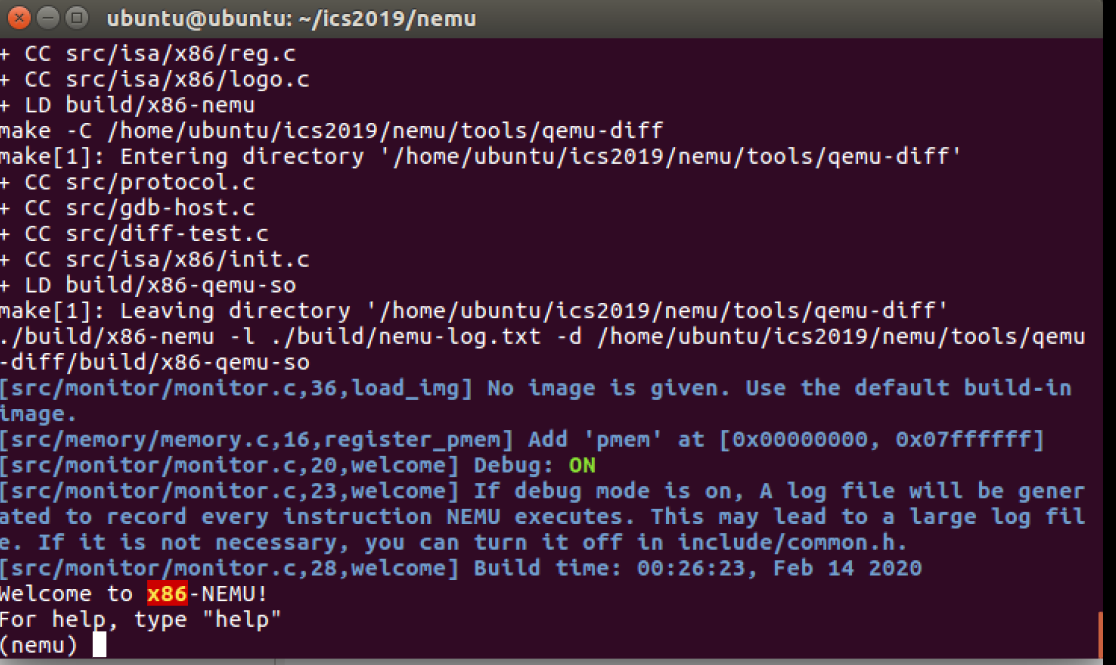
\includegraphics[scale=0.45]{fig/1.png}
        \caption{x86寄存器}
    \end{figure}
}
%——————————————————————————————————————
\subsection{基础设施实现}
\kt{
    经过了对x86isa的寄存器结构实现,NEMU已经可以正常运行,但为了实现提升开发效率的基础设施,我们需要从简单的几个入手并熟悉代码框架:单步执行、打印寄存器状态、扫描内存。

    所需要实现的monitor调试功能均在nemu/src/monitor/debug/ui.c中,我们需要去做的仅仅只是把已有框架下的既定功能实现并完善。

    ui\_mainloop会通过readline()获取控制台的键入命令并使用strtok(跟据第二个参数将第一个参数传入的字符串进行分解并返回第一个子字符串)识别和解析命令,由于简易调试器中的命令如果跟有参数会与前面的命令指示符以空格划分,所以可以使用strtok(str, " ")来获取命令字符串,并将其与cmd\_table中的内容相对比,若有可以匹配的已实现命令则调用命令处理函数,否则报错。
}
%——————————————————————————————————————
\subsubsection{单步执行}
\kt{
    单步执行的实现非常简单,因为框架中已经包含了一个cmd\_c的继续执行函数,我们只要仿照它的实现进行实现即可。即使用cpu\_exec()函数,该函数是模拟CPU,参数表示执行几条指令。同时还要在cmd\_table里面加入相应描述字段和函数handler。实验指导书的sscanf函数很是好用,它是将第一个参数格式化为第二个参数的形式,并以引用的格式将值传递给第三个参数。
    \begin{lstlisting}[title=单步执行,frame=trbl,language={C++}]
        //nemu/src/monitor/debug/ui.c 
        static int cmd_si(char *args){
            int step=0;//单步执行的步数
            /* extract the first argument */
            char *arg = strtok(NULL, " ");//获取N
            if(arg==NULL)//si等价si 1
                cpu_exec(1);
            else {
                sscanf(arg,"%d",&step);//atoi
                if(step<=0)
                    printf("Invalid number!\n");
            else
                cpu_exec(step);//不要使用for循环
            }   
            return 0;
        }
    \end{lstlisting}
    \begin{figure}[H]
        \centering
        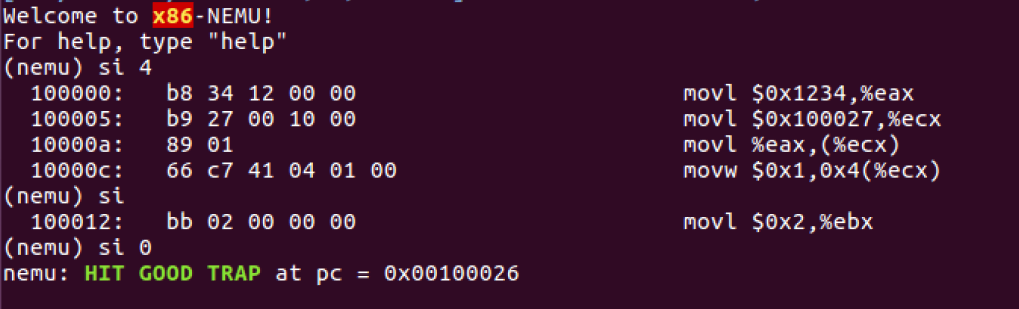
\includegraphics[scale=0.45]{fig/2.png}
        \caption{单步执行si}
    \end{figure}
}
%——————————————————————————————————————
\subsubsection{打印寄存器}
\kt{
    ics2019因为引入了三种不同的ISA所以这一项要在选定的ISA中实现为API,这样就可以屏蔽ISA之间的差异。借助前面构建好的寄存器结构循环输出其中的内容即可。
    \begin{lstlisting}[title=打印寄存器,frame=trbl,language={C++}]
        //nemu/src/monitor/debug/ui.c 
        static int cmd_info(char *args){
            /* extract the first argument */
            char *arg = strtok(NULL, " ");//判断r还是w
            if(strcmp(arg,"r")==0)//info r
                isa_reg_display();//调用reg.c中的API  
            else if(strcmp(arg,"w")==0){
                printf("PA1.1 haven't implement this function yet.");
            }
            else   //没有键入r或w参数
                printf("Unknown command:%s\n",arg);  
            return 0;
        }
        //nemu/src/isa/x86/reg.c
        void isa_reg_display() {
            for(int i=0;i<8;i++)//8个32-bit reg
                printf("%s:\t0x%08x\t\n",regsl[i],cpu.gpr[i]._32);
            for(int i=0;i<8;i++)//8个16-bit reg
                printf("%s:\t    0x%4x\t\n",regsw[i],cpu.gpr[i]._16);
            for(int i=0;i<8;i++)//8个8-bit reg
                printf("%s:\t      0x%02x\t\n",regsb[i],cpu.gpr[i%4]._8[i/4]);
            printf("eip:\t0x%08x\t\n",cpu.pc);//eip
        }
    \end{lstlisting}
    \begin{figure}[H]
        \centering
        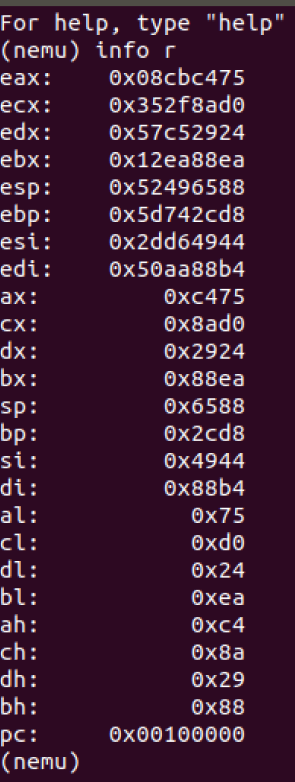
\includegraphics[scale=0.5]{fig/3.png}
        \caption{打印寄存器info r}
    \end{figure}
}
%——————————————————————————————————————
\subsubsection{扫描内存}
\kt{
    阶段一的扫描内存相对简单,只需要对16进制地址向后相应扫描就可以,函数主要是利用了vaddr\_read来读指定地址的内容,阶段一只需要将地址传入并把长度调为4字节就可以了。虽然这个函数写的是vaddr线性地址,但是实际上它在memeory.h被定义为isa\_vaddr\_read,即根据不同ISA调用不同的读取API,但是找到nemu/src/isa/x86/mmu.c中的定义,实际返回的还是paddr\_read的结果,即物理地址的结果。
    \begin{lstlisting}[title=扫描内存,frame=trbl,language={C++}]
        //nemu/src/monitor/debug/ui.c 
        static int cmd_x(char *args){
            /*PA1.1Simple version EXPR must be a hex number,
            such as x 10 0x100000*/
            //use memory/memory.c paddr_read which needs addr and len
            /* extract the first argument */
            int N,start;
            vaddr_t temp;
            char *arg0 = strtok(NULL, " ");//get N,4N
            char *arg1 = strtok(NULL, " ");//get EXPR ,where to start
            if(arg0==NULL||arg1==NULL){
                printf("Lack of parameter!\n");return 0;}
            if(N==0){printf("Invalid parameter!\n");return 0;}
            sscanf(arg0,"%d",&N);
            if(arg1[0]!='0'){//not 0x  hex address
                //PA1.2
            }
            else{
                sscanf(arg1,"%x",&start);
                printf("address\tdata");
                for(int i=0;i<N;i++){
                    if(i%4==0) 
                    printf("\n0x%x:\t0x%02x\t",start+i,vaddr_read(start+i,1));
                    else 
                        printf("0x%02x\t",vaddr_read(start+i,1));
                }
            }
            printf("\n");
            return 0;
        }
    \end{lstlisting}

    NEMU运行结果如下,与src/isa/x86init.c中的默认镜像相对比一致说明功能实现正确。
    \begin{figure}[!h]
        \begin{minipage}[h]{0.5\linewidth}
        \centering
        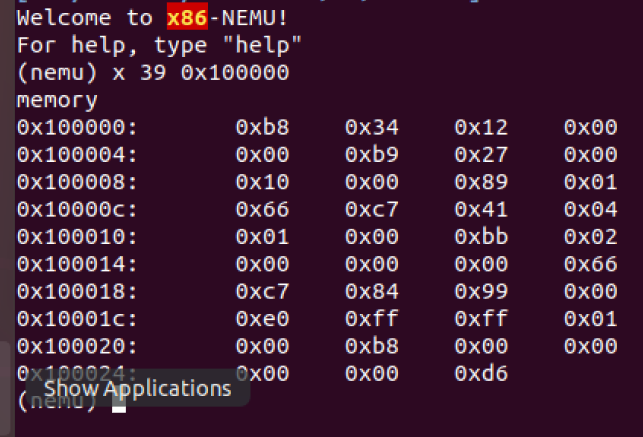
\includegraphics[scale=0.35]{fig/4.png}
        \caption{扫描内存1.0}
        \end{minipage}%
        \hfill
        \begin{minipage}[h]{0.5\linewidth}
        \centering
        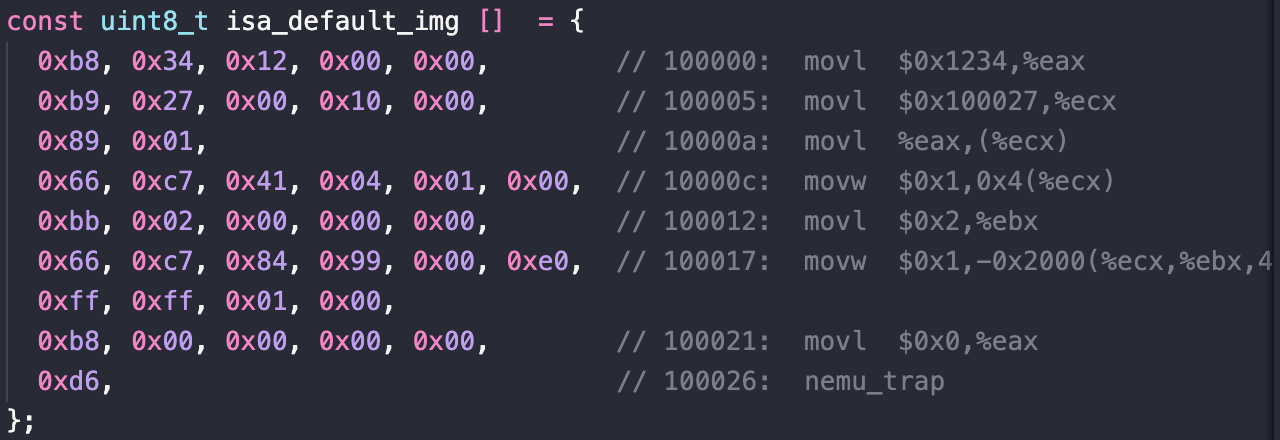
\includegraphics[scale=0.33]{fig/5.png}
        \caption{与默认镜像对比}
        \end{minipage}
    \end{figure}
}
%---------------------------------------------------------------------------------------------------
\section{阶段二}
%——————————————————————————————————————
\subsection{表达式词法分析}
\kt{
    再进行表达式运算之前,首先需要识别出表达式中的token单元,即编译原理中的词法分析阶段。在表达式计算的这一部分只需要实现基本四则运算并忽略空格即可。
    \begin{lstlisting}[title=词法分析,frame=trbl,language={C++}]
        //nemu/src/monitor/debug/expr.c
        enum {TK_NOTYPE = 256, TK_EQ,TK_NEQ,TK_REG,TK_DEC,TK_HEX,TK_NEG,
        TK_AND,TK_OR,TK_LS,TK_RS,TK_LE,TK_GE,TK_POI};
        //rules
        {" +", TK_NOTYPE},    // spaces
        {"0x[0-9A-F][0-9A-F]*", TK_HEX},         // hex
        {"[0-9]|[1-9][0-9]*", TK_DEC},         // dec
        {"\\+", '+'},         // plus
        {"\\-", '-'},         // minus
        {"\\*", '*'},         // multiple
        {"\\/", '/'},         // divide
        {"\\(", '('},         // LB
        {"\\)", ')'},         // RB
        //之后在make_tokens中把token存到tokens数组中
        if(rules[i].token_type==TK_NOTYPE) continue;//忽略空格
        memset(tokens[nr_token].str,'\0',32); //避免溢出
        strncpy(tokens[nr_token].str,substr_start,substr_len);
        tokens[nr_token].type=rules[i].token_type;
        nr_token++;
        break;
    \end{lstlisting}
    第一步词法分析结束后可以看到NEMU已经可以正常输出词法分析的结果了
    \begin{figure}[H]
        \centering
        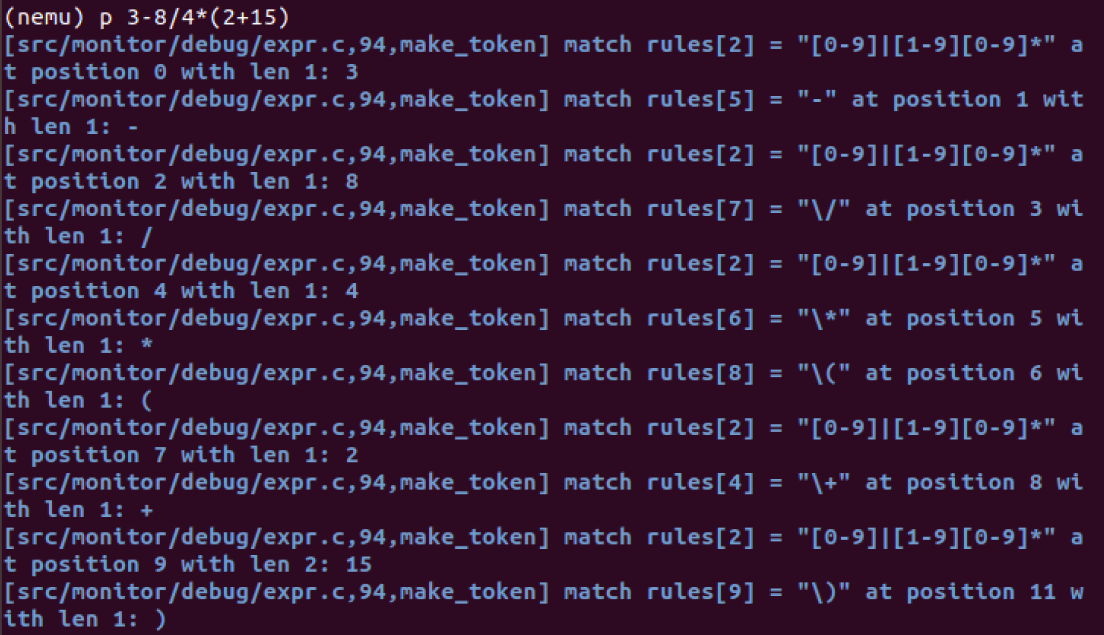
\includegraphics[scale=0.45]{fig/6.png}
        \caption{打印寄存器info r}
    \end{figure}
}
%——————————————————————————————————————
\subsection{递归求值}
\kt{
%——————————————————————————————————————
\subsubsection{括号匹配}
    递归求值的部分可以对应于编译原理的语法及语义分析,首先要对特殊符号“()”进行处理即检查括号配对情况是否正确,我使用了一种比较直观的方法,即将左括号标记为1右括号标记为-1,那么整个表达式最终的加和应该为0才是一个正确的可以进行运算的表达式。
    \begin{lstlisting}[title=括号匹配,frame=trbl,language={C++}]
        //nemu/src/monitor/debug/expr.c
        bool check_parentheses(int p,int q){
        //pq表示表达式字符串的起始和结束位置
        int sum =0;   //sum最终为0 表示表达式括号可全部匹配
        if(!(tokens[p].type=='('&&tokens[q].type==')')) 
            return false;
        else{
            for(int i=p;i<q;i++)
            {
                if(tokens[i].type=='(') sum++;
                else if(tokens[i].type==')') sum--;
                if(sum==0) return false;
                // 在迭代到最后一个符号前如果为0则说明匹配错误
            }
            sum--;//把q的)算上
            if(sum==0) 
                return true;
            return false;
            }
        }
    \end{lstlisting}
%——————————————————————————————————————
\subsubsection{主运算符}
    之后的寻找主运算符的部分可以比作建立语法树,只需要对各个运算符的优先级进行标注即可。下附代码是监视点之后的完整版。
    \begin{lstlisting}[title=主运算符获取及计算,frame=trbl,language={C++}]
    //nemu/src/monitor/debug/expr.c
    uint32_t eval(int p,int q){
        if(p>q) return 0;//错误参数!
        else if(p==q)  //只有一个token的情况:hex dec reg
        {
            uint32_t res;
            if(tokens[p].type==TK_HEX) sscanf(tokens[p].str,"%x",&res);//16进制
            else if(tokens[p].type==TK_DEC) sscanf(tokens[p].str,"%d",&res);//10进制
            else if(tokens[p].type==TK_REG){//寄存器
                char temp[3]={tokens[p].str[1],tokens[p].str[2],tokens[p].str[3]};
                //去掉寄存器前的$
                for(int i=0;i<8;i++)  //32bit
                    if(!strcmp(temp,regl[i])) return cpu.gpr[i]._32; 
                for(int i=0;i<8;i++) //16bit
                    if(!strcmp(temp,regw[i])) return cpu.gpr[i]._16;
                for(int i=0;i<8;i++)  //8bit
                    if(!strcmp(temp,regb[i])) return cpu.gpr[i%4]._8[i/4];  
                if(strcmp(temp,"eip")) return cpu.pc; //eip
            }
            else assert(0);
            return res;
        }
        else if(check_parentheses(p,q)) //检查括号是否匹配
            return eval(p+1,q-1); //是则去掉括号计算括号内部
        else  //找中心算符的部分
        {
            int op=0,prev=10;//优先级
            bool lp=false;//标记左括号
            for(int i=p;i<=q;i++)
            {
                if(tokens[i].type==')'){lp=false;continue;}
                if(lp) continue;
                if(tokens[i].type=='('){lp=true;continue;}
                switch(tokens[i].type)  //prev越大优先级越高
                {
	                case TK_OR:if(prev>1){prev=1;op=i;continue;}
	                case TK_AND:if(prev>2){prev=2;op=i;continue;}
	                case TK_NEQ:if(prev>3){prev=3;op=i;continue;}
	                case TK_EQ:if(prev>3){prev=3;op=i;continue;}
	                case TK_LE:if(prev>4){prev=4;op=i;continue;}
	                case TK_GE:if(prev>4){prev=4;op=i;continue;}
	                case '<':if(prev>4){prev=4;op=i;continue;}
	                case '>':if(prev>4){prev=4;op=i;continue;}
	                case TK_LS:if(prev>5){prev=5;op=i;continue;}
	                case TK_RS:if(prev>5){prev=5;op=i;continue;}
                        case '+':if(prev>6){prev=6;op=i;continue;}
                        case '-':if(prev>6){prev=6;op=i;continue;}
                        case '*':if(prev>7){prev=7;op=i;continue;}
                        case '/':if(prev>7){prev=7;op=i;continue;}
	                case '!':if(prev>8){prev=8;op=i;continue;}
                        case TK_NEG:if(prev>9){prev=9;op=i;continue;}
	                case TK_POI:if(prev>9){prev=9;op=i;continue;}
	                default:continue;
                }
            }
            uint32_t val1=eval(p,op-1);
            uint32_t val2=eval(op+1,q);
            switch(tokens[op].type)    //计算
            {
                case TK_OR:return val1||val2;
                case TK_AND:return val1&&val2;
                case TK_NEQ:return val1!=val2;
                case TK_EQ:return val1==val2;
                case TK_LE:return val1<=val2;
                case TK_GE:return val1>=val2;
                case '<':return val1<val2;
                case '>':return val1>val2;
                case TK_LS:return val1<<val2;
                case TK_RS:return val1>>val2;
                case '+':return val1 + val2;
                case '-':return val1 - val2;
                case '*':return val1 * val2;
                case '/':return val1 / val2;
                case '!':return !val2;
                case TK_NEG:return -1*val2;
                case TK_POI:return vaddr_read(val2,4);
                default:assert(0);
            }
        }
    }

    //nemu/src/monitor/debug/expr.c——expr函数调用即可
    return eval(0,nr_token-1);
    \end{lstlisting}

    之后再在ui.c中完善cmd\_p函数即可
    \begin{lstlisting}[title=表达式计算,frame=trbl,language={C++}]
    ////nemu/src/monitor/debug/ui.c
    static int cmd_p(char *args){
        bool success=false;
        //char *arg = strtok(NULL, " ");//注释掉是因为expr中可能有空格
        if(args==NULL){printf("Lack of parameter!\n");return 0;}
        uint32_t res=expr(args,&success);
        printf("Decimal:%u  Hex:0x%x\n",res,res);
        return 0;
    }
    \end{lstlisting}
%——————————————————————————————————————
\subsubsection{负数}
    此时指导书又提出了新的刁难?负数的实现,难点在于分裂减号和负号,要正确判断负号的出现,之后对负号进行标记并使其获得最高优先级即可。不是很懂为什么要做负数,指导书写的是你迟早会面临类似的问题,所以做了,但是后面的随机测试又要求无符号整型,所以在cmd\_p中的输出就写成了\%u。然后过了几天老师发了等价于参考代码和样例的指导书,于是我又把\%d改了回去,负数仍显示负数,毕竟我还有个Hex十六进制的表示。
    \begin{lstlisting}[title=负数,frame=trbl,language={C++}]
        //nemu/src/monitor/debug/expr.c
        {"-", '-'},         // minus 识别token处
        //对于负号优先度的处理前面代码以及有过就不再赘述
        //在expr函数中进行标记
        if(nr_token!=1)//只有一个符号的时候不用区分
            for(int i=0;i<nr_token;i++)//检查负号还是减号
                if(tokens[i].type=='-'&&(i==0||tokens[i-1].type=='('||
                tokens[i-1].type==TK_NEG||tokens[i-1].type=='-'
                ||tokens[i-1].type=='+'||tokens[i-1].type=='*'
                ||tokens[i-1].type=='/'))
                    tokens[i].type=TK_NEG;
                    //第一个符号、左边为(、负号后跟+-*/的时候都标记为负号
    \end{lstlisting}
    \begin{figure}[!h]
        \begin{minipage}[h]{0.5\linewidth}
        \centering
        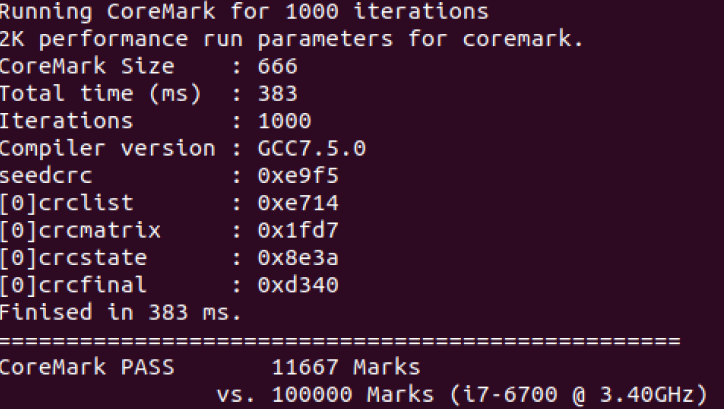
\includegraphics[scale=0.18]{fig/14.png}
        \caption{负数无符号}
        \end{minipage}%
        \hfill
        \begin{minipage}[h]{0.5\linewidth}
        \centering
        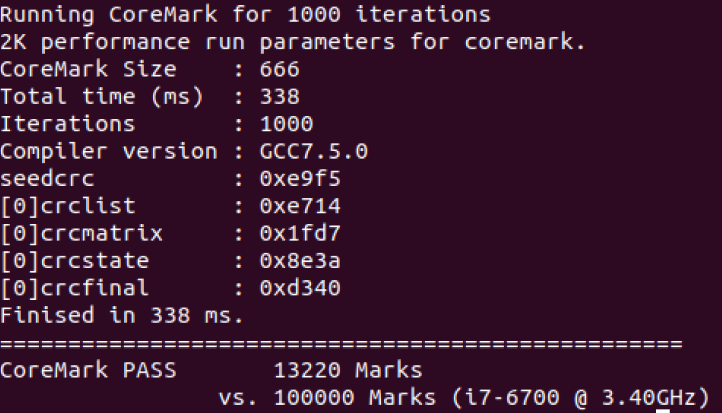
\includegraphics[scale=0.3]{fig/15.png}
        \caption{负数有符号}
        \end{minipage}
    \end{figure}

    到此整个表达式求值的阶段二就算是功能实现完成了,验证结果如下:
    \begin{figure}[!h]
        \begin{minipage}[h]{0.5\linewidth}
        \centering
        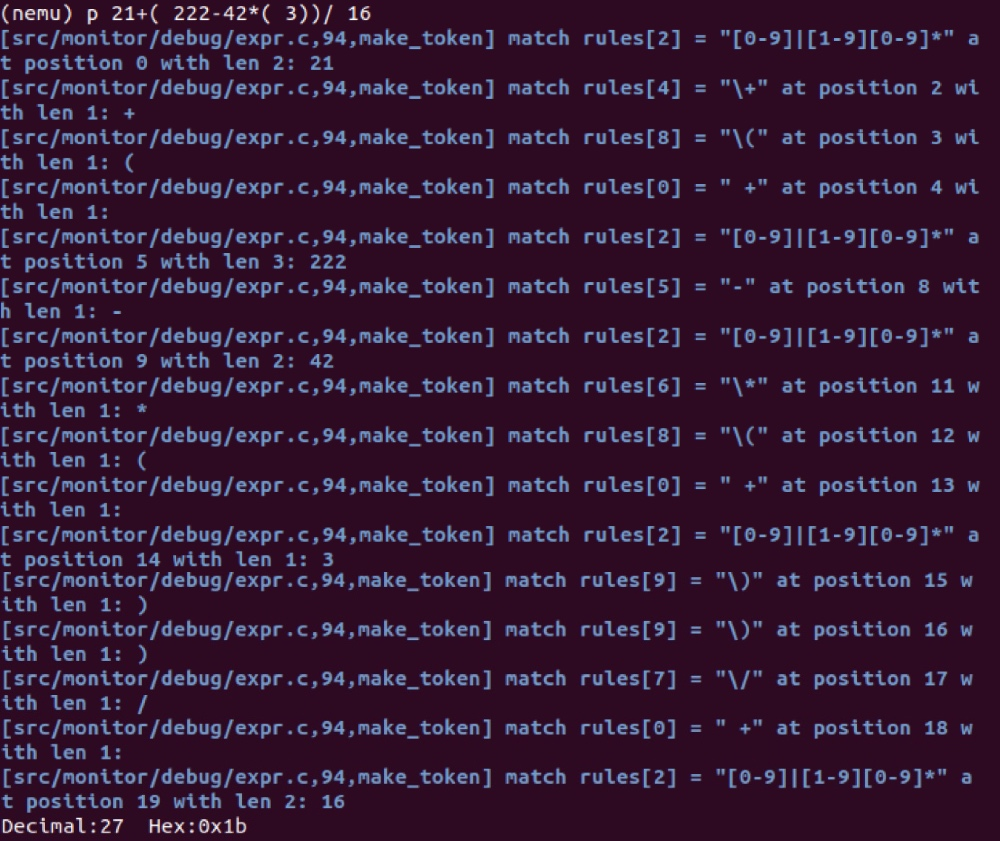
\includegraphics[scale=0.15]{fig/7.jpg}
        \caption{验证1}
        \end{minipage}%
        \hfill
        \begin{minipage}[h]{0.5\linewidth}
        \centering
        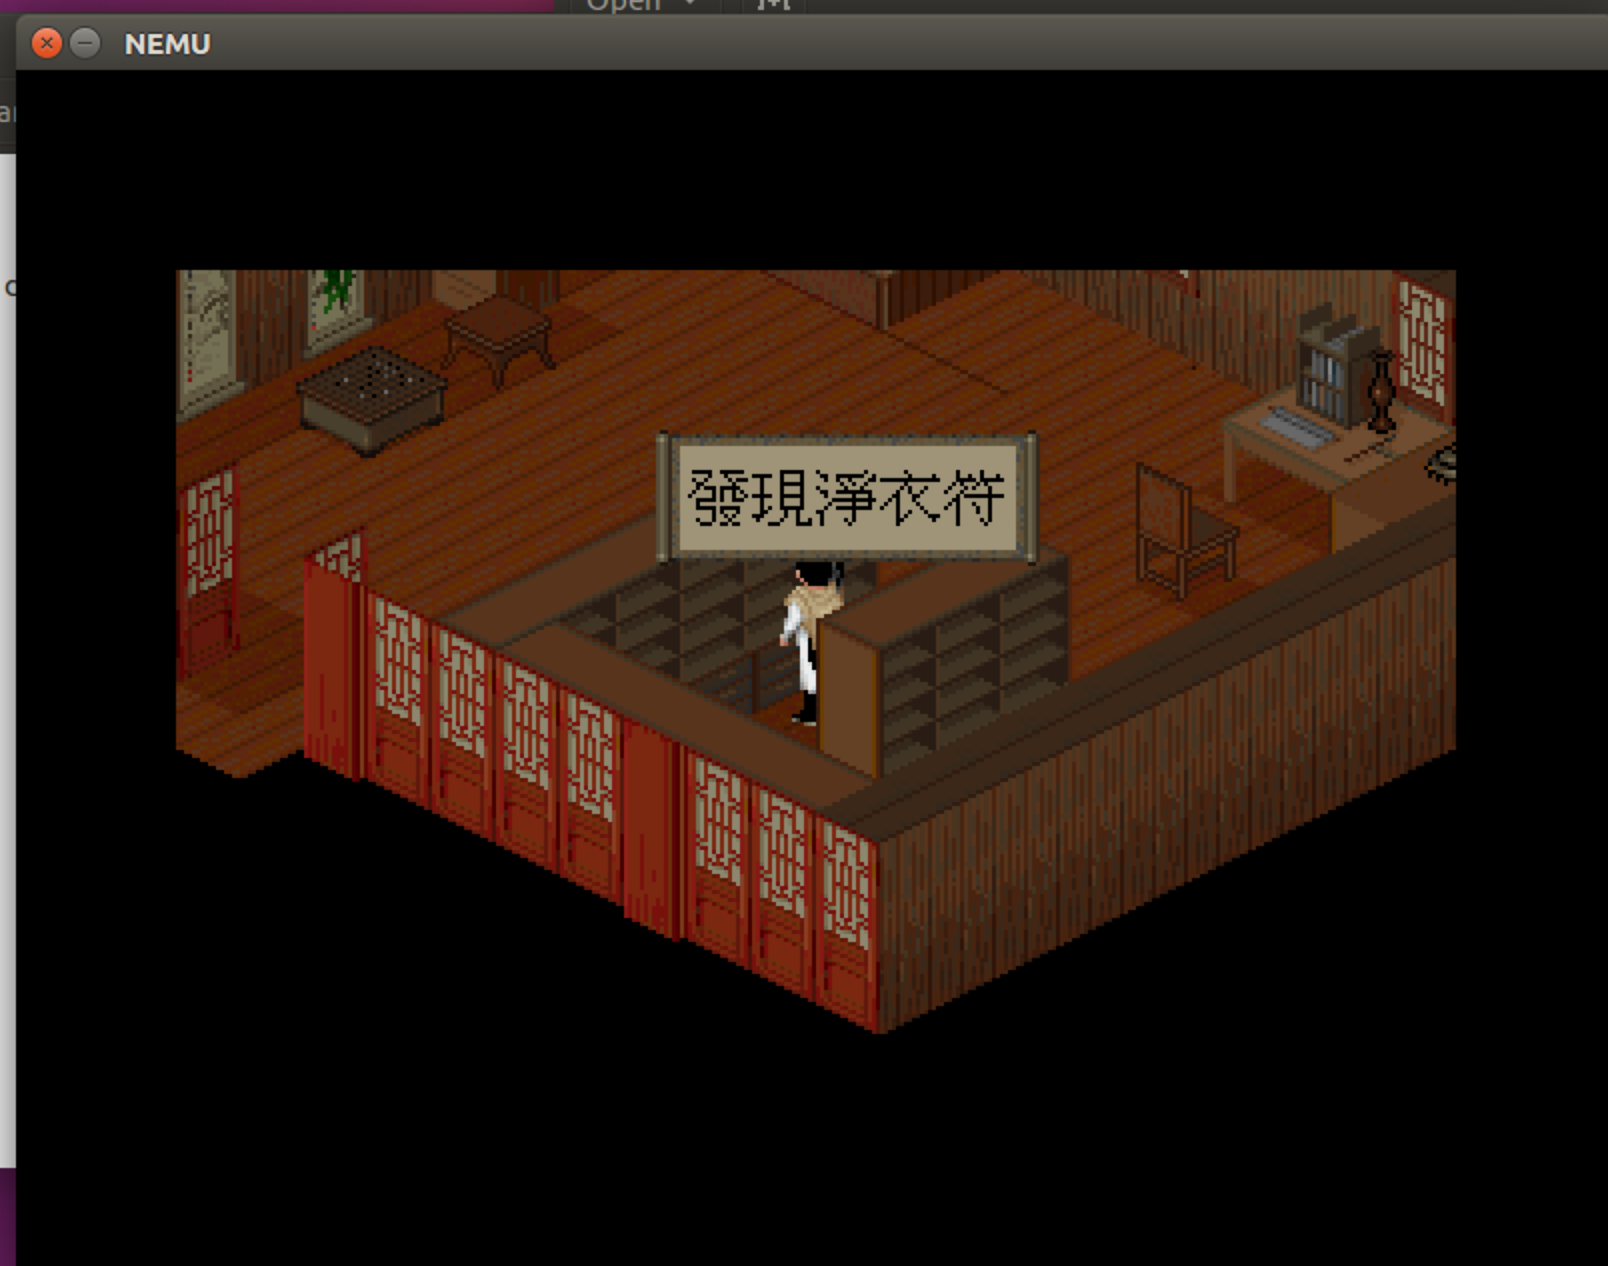
\includegraphics[scale=0.3]{fig/8.png}
        \caption{验证2}
        \end{minipage}
    \end{figure}
%——————————————————————————————————————
\subsubsection{随机测试}
    于是又有了新的难题,老师给的代码里并没有nemu/tools文件夹,但是ics2019代码中是有的,所以还是想尝试着做一下,但是差不多就好像是为了测试前一个程序的bug写了另一个更大的bug。

    框架也是事先做好的,只需要补充代码就可以了,整体上没有理解的难度。
    \begin{lstlisting}[title=随机测试,frame=trbl,language={C++}]
        //nemu/tools/gen-expr/gen-expr.c
        static char buf[65536]="";  //init
        int prob[10]={0,0,1,1,2,2,2,2,2,2};
        //因为直接用rand均匀分布效果不好,为增加复杂性手动调整概率
        static inline void gen_rand_op(){//随机生成运算符
            switch(rand()%4){
                case 0:{strcat(buf,"+");break;}
                case 1:{strcat(buf,"-");break;}
                case 2:{strcat(buf,"*");break;}
                case 3:{strcat(buf,"/");break;}
                default:assert(0);
            } 
        }
        static int sign=0;//记录迭代次数
        static inline void gen_rand_expr() {//随机生成表达式
            if (sign>50){return;}
            sign++;
            switch(prob[rand()%10]){//0数字1括号2复杂表达式拼接(包含1、2)
                case 0:{char s[4];int a=rand()%10;while(a==0)a=rand()%10;
                    while(prob[rand()%10]) 
                        a+=rand()%10;sprintf(s,"%d",a);strcat(buf,s);break;}
                case 1: {if(prob[rand()%10])strcat(buf," ");strcat(buf,"(");
                if(!prob[rand()%10])strcat(buf," ");gen_rand_expr();
                if(!prob[rand()%10])strcat(buf," ");strcat(buf,")");break;}
                default:{if(!prob[rand()%10])strcat(buf," ");
                gen_rand_expr();if(!prob[rand()%10])strcat(buf," ");
                gen_rand_op();if(!prob[rand()%10])strcat(buf," ");
                gen_rand_expr();break;}
            }
        }
        //使用sprintf写到文件中的时候加了判断,除数为0则continue
        //之后在main中调用并注意清0即可
    \end{lstlisting}
    \begin{figure}[H]
        \centering
        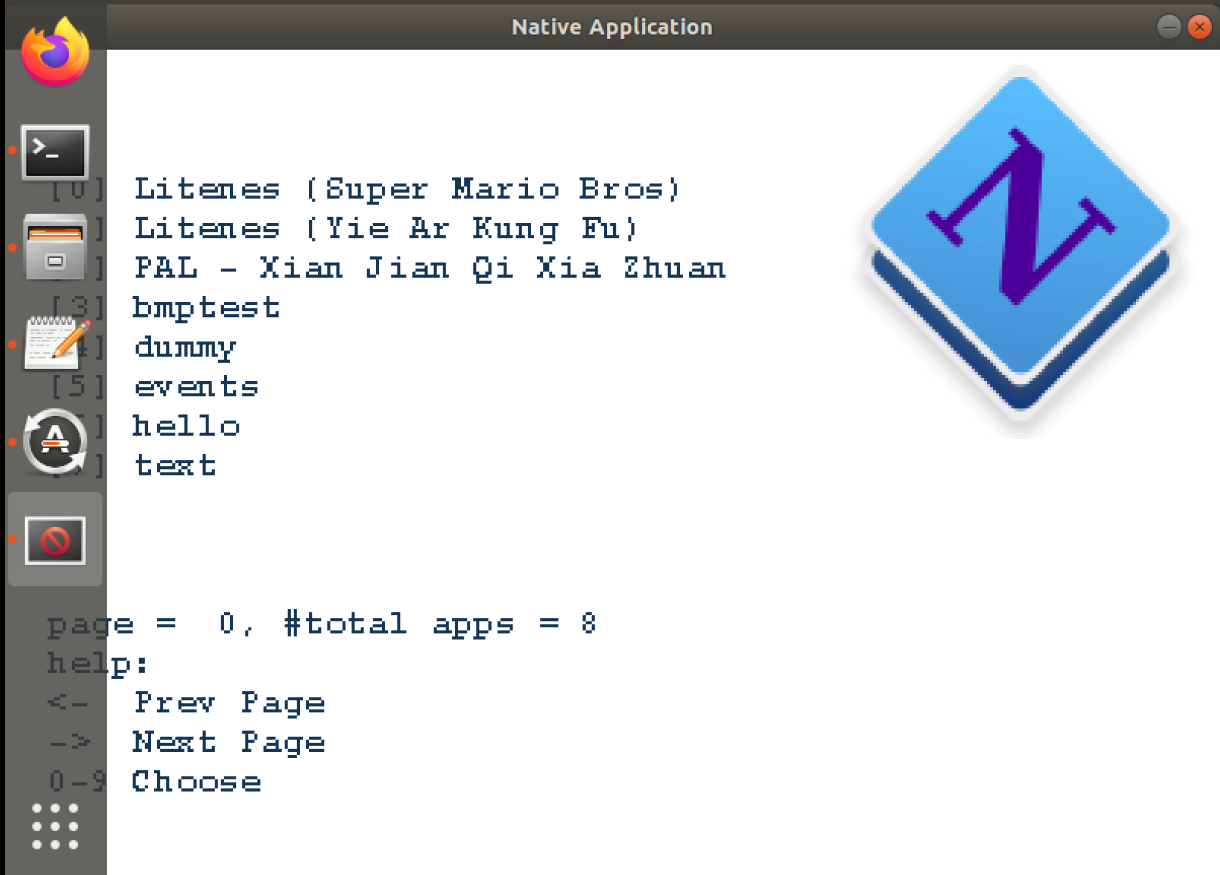
\includegraphics[scale=0.45]{fig/9.png}
        \caption{随机测试input}
    \end{figure}

    之后再对NEMU的main.c进行相应修改就可以让NEMU一启动起来就进行自动计算input提供的算术表达式并与答案相对比输出结果。
    \begin{lstlisting}[title=随机测试,frame=trbl,language={C++}]
        //nemu/src/main.c
        //添加头文件
        #include <stdio.h>
        #include <stdlib.h>
        #include <string.h>
        #include "monitor/expr.h"
        //to test p EXPR
        FILE*fp;
        fp=fopen("/home/ubuntu/ics2019/nemu/tools/gen-expr/input","r");
        char buf[101];
        while(fgets(buf,sizeof(buf),fp)){
            char *p=strtok(buf," ");
            char *q=strtok(NULL,"\n");
            bool success=true;
            int res=expr(q,&success);
            if(success){
                if(atoi(p)==res){
                    printf("%s=%s, myresult=%d, equal=true\n",q,p,res);}
                else {printf("%s=%s, myresult=%d, equal=false\n",q,p,res);}
            }
            else {printf("fail to eval");}
        } 
        fclose(fp); 
    \end{lstlisting}
    \begin{figure}[H]
        \centering
        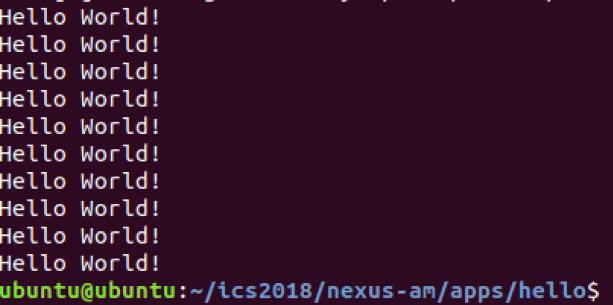
\includegraphics[scale=0.45]{fig/10.png}
        \caption{随机测试验证结果}
    \end{figure}

    其实整体来说,随机测试并没有严格意义上的完整实现,因为有几个小细节被我skip了,以及学姐的段错误解决等详细想法见问题与解决。

    之后再将表达式的部分加入到前面扫描内存当中实现完整的功能
    \begin{lstlisting}[title=扫描内存2.0,frame=trbl,language={C++}]
        //nemu/src/monitor/debug/ui.c       cmd_x
        if(arg1[0]!='0'){//not 0x  hex address
            bool success=true;
            temp=expr(arg1,&success);
            if(!success){printf("Illegal Address!\n");return 0;}
        }
    \end{lstlisting}
    \begin{figure}[H]
        \centering
        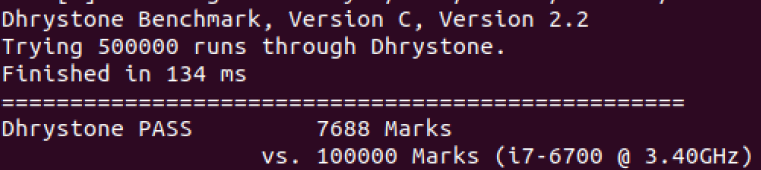
\includegraphics[scale=0.45]{fig/12.png}
        \caption{扫描内存2.0}
    \end{figure}
}
%---------------------------------------------------------------------------------------------------
\section{阶段三}
%——————————————————————————————————————
\subsection{扩展表达式功能}
\kt{
    在前面阶段二实现的基础上对优先级处理以及token添加即可,唯一需要注意的是指针的*和负号的处理一样也是需要进行区分的
    \begin{lstlisting}[title=指针,frame=trbl,language={C++}]
        //nemu/src/monitor/debug/expr.c
        for(int i=0;i<nr_token;i++)
            if(tokens[i].type=='*'&&(i==0||(tokens[i-1].type!=TK_DEC 
            && tokens[i-1].type!=TK_HEX && tokens[i-1].type!=')')))
                tokens[i].type=TK_POI;
    \end{lstlisting}

    然后很久以后老师又给了测试样例,(麻烦老师下次给早一点QAQ),不过也多亏老师的测试样例我才发现我的十六进制数正则表达式只认大写字母,于是我又替换了一次图片为测试样例。
    \begin{figure}[!h]
        \begin{minipage}[h]{0.5\linewidth}
        \centering
        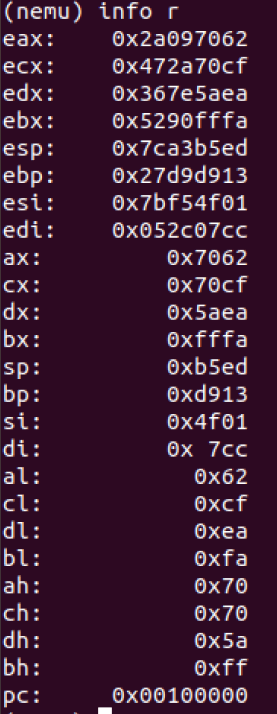
\includegraphics[scale=0.45]{fig/23.png}
        \caption{此时的寄存器对应以验证正确性}
        \end{minipage}%
        \hfill
        \begin{minipage}[h]{0.5\linewidth}
        \centering
        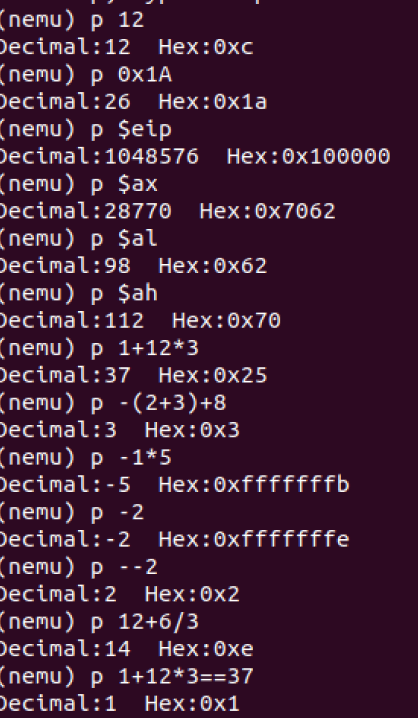
\includegraphics[scale=0.4]{fig/24.png}
        \caption{测试样例1}
        \end{minipage}
    \end{figure}
    \begin{figure}[H]
        \centering
        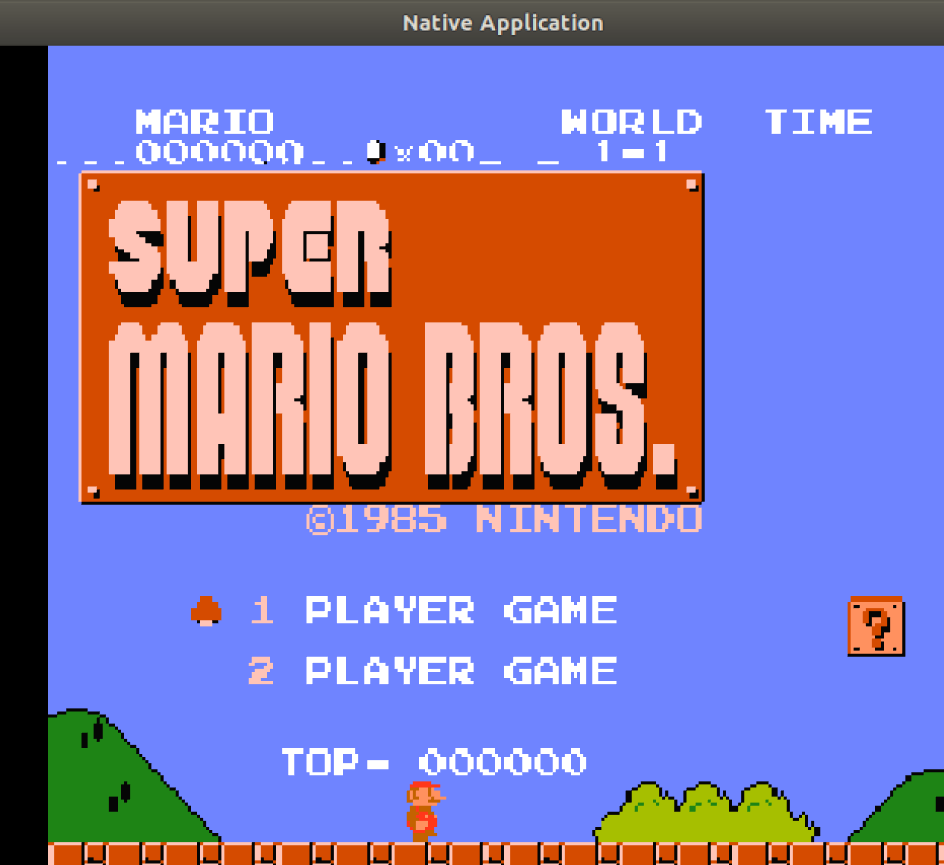
\includegraphics[scale=0.45]{fig/22.png}
        \caption{测试样例2}
    \end{figure}
}
%——————————————————————————————————————
\subsection{实现监视点}
\kt{
    首先需要在nemu/include/monitor/watchpoint.h中完善wp\_pool结构,之后再分别实现创建监视点,查看监视点以及删除监视点的成员函数即可。
    \begin{lstlisting}[title=指针,frame=trbl,language={C++}]
        //nemu/include/monitor/watchpoint.h
        typedef struct watchpoint {
            int NO;
            struct watchpoint *next;
            uint32_t init;//旧值
            char wpexpr[100];//expr
            int hit;//触发次数

        } WP;
        WP* new_wp();//找到一个空闲的监视点
        void free_wp(int no);//释放
        void view_wp();//查看
        bool check_wp();//检查
        void set_wp(char *args);//建立
        //nemu/src/monitor/debug/watchpoint.c
        void init_wp_pool() {
            int i;
            for (i = 0; i < NR_WP; i ++) {
                wp_pool[i].NO = i;
                wp_pool[i].next = &wp_pool[i + 1];
                wp_pool[i].init=0;//初始化
                wp_pool[i].hit=0;//初始化
            }
            wp_pool[NR_WP - 1].next = NULL;
            head = NULL;
            free_ = wp_pool;
}
        WP* new_wp(){
            if(head == NULL){
                head = free_;//直接从free中拿
                free_=free_->next;
                head->next = NULL;
                return head;
            }
            else{
                if(free_ == NULL) //无空闲
                    assert(0);
                WP* temp = head;
                while(temp->next!=NULL)
                    temp = temp->next;
                temp->next = free_;
                free_ = free_->next;
                temp = temp->next;
                temp->next = NULL;
                return temp;
            }
        }
        void free_wp(int no){//释放到free_中
            WP *wp=head;
            while(wp!=NULL){
                if(wp->NO == no)break;
                wp = wp->next;
            }
            if(wp == NULL){
                printf("Fail to free the wp"); 
                return;
            }
            if(head == wp)  head = head->next;
            else{
                WP* temp = head;
                while(temp!=NULL){
                    if(temp->next == wp){
                        temp->next = wp->next;
                        break;
                    }
                    temp = temp->next;
                }
            }
            wp->next = free_;
            free_ = wp;
        }
        void view_wp(){
            if(head==NULL) {printf("no watchpoint now!\n");}
            else{
                printf("NO\tExpr\tHit\n");
                WP *temp = head;
                while(temp!=NULL){
                    printf("%d\t%s\t%d\n",temp->NO,temp->wpexpr,temp->hit);
                    temp = temp->next;
                }
            }
        }
        bool check_wp(){  //监视点有变动返回true
            WP *temp = head;
            while(temp!=NULL) {
                bool *success = false;
                uint32_t new_val = expr(temp->wpexpr,success); 
                if(new_val != temp->init){
                    printf("Watchpoint %d: %s\n",temp->NO,temp->wpexpr);
                    printf("Old value = %d\nNew value = %d\n",
                    temp->init,new_val);
                    temp->init = new_val;//赋新值
                    return false;
                }
                temp = temp->next;
            }
            return true;
        }
        void set_wp(char *args){
            WP* newwp=new_wp();
            strcpy(newwp->wpexpr,args);
            bool *success = false;
            newwp->init=expr(newwp->wpexpr,success);
            printf("Set watchpoint %d on %s successfully\n",
            newwp->NO,newwp->wpexpr);
        }
    \end{lstlisting}

    之后再在ui.c中调用函数即可实现监视点功能,同时在cpu\_exec.c中加入check\_wp的内容即可实现监视点完整功能
    \begin{lstlisting}[title=监视点ui,frame=trbl,language={C++}]
        //nemu/src/monitor/debug/ui.c
        static int cmd_w(char *args){//设置监视点
            if(args==NULL){printf("Lack of parameter!\n");return 0;}
            set_wp(args);
            return 0;
        }
        static int cmd_d(char *args){//删除监视点
            if(args==NULL){printf("Lack of parameter!\n");return 0;}
            int num;
            sscanf(args,"%d",&num);
            if(num<0){printf("Enter a positive number!\n");return 0;}
            free_wp(num);
            printf("Delete watchpoint %d successfully\n",num);
            return 0;
        }
        static int cmd_info(char *args){//  info w补充完善
            char *arg = strtok(NULL, " ");//get r or w
            if(strcmp(arg,"r")==0)//info r
                isa_reg_display();//reg.c API  
            else if(strcmp(arg,"w")==0){
                view_wp();
            }
            else
                printf("Unknown command:%s\n",arg);
            return 0;
        }
        //nemu/src/monitor/cpu_exec.c
        //找到写着TODO check watchpoint的地方
        if(check_wp()==false)
            nemu_state.state=NEMU_STOP;
        /*这里2019的代码和老师提供的2018不一样,因为
        nemu_state在2019是个包含终止pc和ret值的结构体表示状态的
        enum状态只是一个成员变量*/
    \end{lstlisting}
    由于我自己写的测试样例又和老师不一样,所以又一次进行了更新
    \begin{figure}[H]
        \centering
        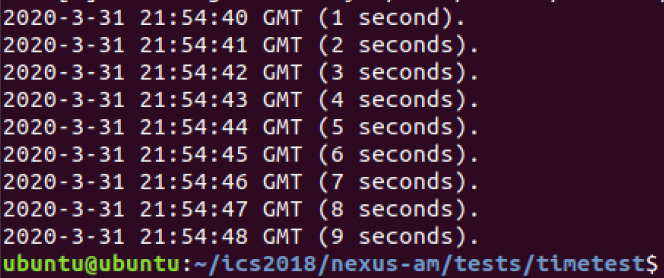
\includegraphics[scale=0.45]{fig/11.png}
        \caption{设置、删除监视点}
    \end{figure}
}
%---------------------------------------------------------------------------------------------------
\section{遇到的bug及解决}
\kt{
    终于完成了PA1的全部内容,从PA0的环境配置到PA1的简易调试器真的是坎坷,没有STFW的帮助真的寸步难行,PA指导书与ucore指导书相比内容有趣了不少,但是同样也有许多挖坑以及故意刁难的感觉,以下是实验过程中遇到的机器和我本人的bug的不完全总结。
    \begin{itemize}
        \item 环境配置PA0
        \begin{todolist}
            \item [\done] Vmware 在32位ubuntu上无法完成与本机之间的复制粘贴,但64位可以。网上给出的解决方案是将vmtools重新安装:\textbf{sudo apt-get autoremove open-vm-tools}\ \ \ \textbf{sudo apt-get install open-vm-tools-desktop},重启虚拟机之后就可以正常复制粘贴但文件拖拽依然只能通过共享文件夹
            \item [\done] 必须要用复制粘贴是因为指导书提供的清华镜像源通过那条命令是更换error的,所以直接上网搜如何更换阿里源,32位和64位以及版本不同会导致系统代号不同,老师提供的32位镜像对应xenial,而我另外配置的最新64位对应bionic。更换镜像之后,所有的apt-get内容不超过2分钟。
            \item [\done] Vim因为用过所以不觉得难受,但是指导书给的例子必须要习惯hjkl代替上下左右确实比较痛苦。\textbf{i1<ESC>q1yyp<C-a>q98@1}这条Vim指令可以一行一个数字从1-100的输出,其含义是i1插入1、yy复制一整行p粘贴ctrl+a(x)是游标下字符+1(-1)、q到q之间是把这部分内容放寄存器、@1重复一次;\textbf{<C-v>24l4jd\$p} 实现文本的左右颠倒,其含义为(确认光标在文本开头)ctrl+v打开可复制view模式、24l光标向右24、4j光标向下4、d\$删除之后所有的p粘贴  
            \item [\done] 直接在32位运行mario是不行的,重新配置ssr和X server也不可以,因为官方18的代码就要求是64位的,会报错。所以32位的对应老师提供的代码,而18或者19的代码在64位机器上运行是没有问题的。
            \item [\wontfix] 将实验环境迁移为MacOS或Windows上的Docker以适应2019的代码 
        \end{todolist}
        \item 阶段一
        \begin{todolist}
            \item [\done] 2019的代码把eip换成了pc,虽然不知道为什么要这么做,但是秉持着不改动无关代码的原则,我只对pc进行了显示上的eip转换。cpu.pc的定义在nemu/src/isa/x86/include/isa/reg.h中,即需要我们进行union定义的地方
            \item [\done] 最开始的在实现si单步执行的时候没有仔细看cpu\_exec的源码,所以执行N步的时候是直接使用的for循环,目前来看是没有问题的,但是到了PA2更新PC用循环就非常有趣了
            \item [\done] 扫描内存最早写的是直接vaddr\_read按长度4字节的去读,但是如果四字节一起读出来,整个内存内容会和期望的default\_img的内容是相反的,因为x86是小端模式,所以在一个一个字节取数据的时候就会先从小端取数,而四个字节四个字节取的话就一个整体取出来,所以将读取变成以1字节为单位读取,这样结果就和预期一致了。
        \end{todolist}
        \item 阶段二
        \begin{todolist}
            \item [\done] 词法分析的时候,声明枚举符号token类型部分,之所以TK\_NOTYPE是从256开始,是为了不与ASCII冲突,但是稍微实验了下,如果将值赋成一些特殊字符的编号也是没有影响的,这一部分要很注重KISS法则,不然后面怎么bug的都定位不了
            \item [\done] 在编译原理当中使用yacc工具编写词法分析的符号只需要一个反斜杠,即\\+就可以了,但是在PA里面却需要两个反斜杠,这个问题的答案是在写报告的时候想到的,就和latex一样,反斜杠本身就是特殊符号,所以还需要一个转义反斜杠来表示出它本身
            \item [\done] cmd\_p的时候习惯性的写了strtok拆分,然后报了挺长的错,后来才想起来expr内部是允许有空格的,一旦拆分会触发自己后面写的一个assert。(典型的自己挖坑)
            \item [\done] 随机测试确实理解和实现都没有难度,但是有一个bug暴露了我的C++代码能力,拼接字符串我第一个想到的是笨拙的使用char*数组,第二个想到的是复杂的用strncpy,错了好久以后才STFW了正确的strcat,太久没写过C++了,完全是试错
            \item [\done] 随机测试有一个很神奇的地方,\textbf{fscanf(fp, "\%d", \&result);}作为一段原有代码,它的本意是读取程序生成的表达式运算结果,但可能由于编译器担心没有assert的部分,不能保证正确性,所以报了error,而报错的原因很简单,是gcc编译器将warning视作error了,参考了一下gen-expr下的makefile,把其中gcc参数的-Werror去掉就行了,虽然这种做法不正确,但是可以最快解决问题
            \item [\done] 按照rand的均匀分布容易让随机表达式总是落在简单和重复括号的区间,所以直接自己写了一个适应程序的概率分布,这样可以更多的生成复杂表达式;还有一个是指导书提出的问题如何处理溢出,通过加入迭代次数终止循环,否则基本上只要开始生成复杂表达式就停不下来;随机空格的实现就是在表达式生成中间通过随机概率插入;
            \item [\wontfix] 保证无符号运算我的理解是\%u输出,但是这并不是理想的结果,那理想的方案是每运算一步即判断是否大于0,不是则舍去表达式;过滤求值中有除0行为的表达式,单纯除0的过滤也已经写到程序中了,表达式中间结果为0作为除数的直接写在了gen-expr中,在输出到文件的时候对这串表达式进行验证,由于规定了无符号,所以为负则可以跳过这次输出到文件。另外学姐的段错误我也报过,第一次是因为除0表达式没有过滤完整,第二次是因为buf溢出,所以每打印完一个表达式对buf进行memset清0即可,同样在代码中使用迭代次数来记录迭代生成表达式的次数,防止迭代次数太多套死自己的情形发生,间接的也避免了buf溢出的情形。
        \end{todolist}
        \item 写完报告很久以后突然在准备做PA2的时候发现PA1的所有内容全都给做到PA0分支去了,于是赶紧悬崖勒马又把代码重新挪了一遍,幸亏我的报告比较详细才能较快的恢复,虽然中间少了许多报错的run的log但是内容还是经检验无误的,也让我彻底记住了开发中分支的重要性,(习惯于自己直接往master提交的严重后果)
    \end{itemize}
}
%---------------------------------------------------------------------------------------------------
\section{思考题\&\&必答题}
%——————————————————————————————————————
\subsection{思考题}
\kt{
    \begin{enumerate}
        \item 如果没有寄存器, 计算机还可以工作吗? 如果可以, 这会对硬件提供的编程模型有什么影响呢?
        
        可以工作,虽然没有了寄存器,但一些操作所依据的数据存储方式一定是要被定义的,一些旧模型下的计算机使用RAM的第一页作为主要暂存空间,因此前256个字节被称为“寄存器”,即使它们是电子意义上的DRAM。虽然可以工作,但效率肯定远低于寄存器。编程模型似乎有个必要条件就是在寄存器中对指令的处理,一周目没有很看懂。
        \item 什么东西表征了TRM的状态? 在状态模型中, 执行指令和执行程序, 其本质分别是什么?
        
        TRM中存在一个叫做状态寄存器的组成部分,会存储图灵机当前的状态。执行指令和执行程序的本质区别是程序是许多指令的集合。此外程序寄存器仅用来存储程序的下一条指令所在地址。
        \item 一个程序从哪里开始执行呢?
        
        一般来说像C/C++这种是从main函数开始执行的,但是汇编语言又似乎可以指定程序的入口地址,所以STFW到\_\_attribute\_\_机制,可以设置入口地址,而gcc是默认设定为main的
        \item 阅读init\_monitor()函数的代码, 你会发现里面全部都是函数调用. 按道理, 把相应的函数体在init\_monitor()中展开也不影响代码的正确性. 相比之下, 在这里使用函数有什么好处呢?
        
        个人理解,方便调试和归类,全用源码替换,就算注释写得再好也会乱七八糟,如果把每一个不同的功能实现放在一个.c文件里,虽然文件变多了,但是条理清晰了,对需要RTFSC的人很友好,对调试也友好
        \item parse\_args这些参数是从哪里来的呢?
        
        当然是main来的,调用逻辑是main→init\_monitor→parse\_args,而main函数的参数是在运行的时候通过控制台输入的
        \item 阅读reg\_test()的代码, 思考代码中的assert()条件是根据什么写出来的.
        
        第一个for循环里面的assert检查32位和16位寄存器,即EAX低16位是否与AX一致;之后一部分验证8位是否与16位对应;最后验证是不是和cpu结构中的一致
        \item 在cmd\_c()函数中, 调用cpu\_exec()的时候传入了参数-1, 你知道这是什么意思吗?
        
        这个问题的答案在nemu/src/monitor/cpu-exec.c中cpu\_exec的定义中,传入参数的类型是uint64\_t,所以-1其实是最大的数0xffffffffffffffff,所以这个for循环可以保证循环最多的次数,可以把所有的命令执行完而不至于说在我指令没有执行完之前程序提前结束
        \item opcode\_table到底是个什么类型的数组?
        
        是一个opcode\_entry结构体类型的数组,通过RTFSC猜测是模拟指令码的结构体
        \item 谁来指示程序的结束?
        
        首先如果主函数里面有exit()的话也会直接结束,c语言中有atexit()函数,如果将一组指向函数的指针传递给atexit()函数,那么在程序退出main()后,就会自动调用该函数;而且main函数返回值以后,操作系统还要根据返回值判断程序正常退出还是异常退出,之后程序才会结束运行;全局对象的析构函数会在main函数之后执行
        \item 阅读nemu/Makefile, 尝试理解NEMU的编译过程. 特别地, NEMU是如何支持多种客户ISA的? 你现在可以忽略这个问题, 但你会在PA2中重新面对它.
        
        这个Makefile相比ucore的真的简单了不少,基本就是包含文件,gcc编译生成,链接,再之后就是run、clean这些的实现。多种ISA,在最一开头就定义了变量ISA ?= x86,需要isa不同的时候调用\$ISA变量即可
        \item 为什么printf()的输出要换行?
        
        不然所有的输出堆在一起吗,看着都难受。如果没有换行,那么缓存会一直填满,溢出是迟早的事情吧。而且这个NEMU只是一个模拟机,我以为他会和bash编译器一样自动换行,然而并没有,扫描内存的时候最后忘了写换行,(nemu)真的就直接跟在后面了。。
        \item 框架代码中定义wp\_pool等变量的时候使用了关键字static, static在此处的含义是什么? 为什么要在此处使用它?
        
        静态全局变量,保证只在定义文件内有效,既有全局变量的功能,也避免了不必要的外部调用。其他源文件必须通过封装函数才可以实现对该变量的操作。
        \item x86的int3指令不带任何操作数, 操作码为1个字节, 因此指令的长度是1个字节. 这是必须的吗? 假设有一种x86体系结构的变种my-x86, 除了int3指令的长度变成了2个字节之外, 其余指令和x86相同. 在my-x86中, 上述文章中的断点机制还可以正常工作吗? 为什么?
        
        不能,因为int3指令长度为1个字节时,且存在想设置断点的指令的第一个字节处,当程序执行到0xcc,就会出发异常进入调试,但当int3指令的长度变为2个字节后,会遇到如下问题:因为x86架构上指令最短的长度就是1字节,这样可以保证只有我们希望停止的那条指令被修改;如果遇到单字节指令,2位长度的 int3 会影响到其他指令; 在运行过程中,按每个字节的内容来解读,改变后的int3指令就会被分开,可能不会正确解读
        \item 如果把断点设置在指令的非首字节(中间或末尾), 会发生什么? 你可以在GDB中尝试一下, 然后思考并解释其中的缘由.
        
        出现段错误
        \item 你已经对NEMU的工作方式有所了解了. 事实上在NEMU诞生之前, NEMU曾经有一段时间并不叫NEMU, 而是叫NDB(NJU Debugger), 后来由于某种原因才改名为NEMU. 如果你想知道这一段史前的秘密, 你首先需要了解这样一个问题: 模拟器(Emulator)和调试器(Debugger)有什么不同? 更具体地, 和NEMU相比, GDB到底是如何调试程序的?
        
        Emulator是用于分析研究目标系统本身,其本身要跟CPU所有内部行为一致,Debugger的最基本功能就是将一个飞速运行的程序中断下来,并且使其按照用户的意愿执行,主要靠异常实现
    \end{enumerate}

    此外还有几个建议二周目思考的题目实在是想不出,STFW没有结果以及不知道往哪个方向RTFM,所以暂时放下。
}
%——————————————————————————————————————
\subsection{必答题}
\kt{
    必答题只有如何阅读手册这部分是需要回答的,其余必答题皆为代码实现。
    \begin{enumerate}
        \item 假设你现在需要了解一个叫selector的概念, 请通过i386手册的目录确定你需要阅读手册中的哪些地方. 即使你选择的ISA并不是x86, 也可以尝试去查阅这个概念.
        
        打开手册ctrl+f查找selector,定位到-CHAPTER 5 MEMORY MANAGEMENT ---5.1.3 Selectors
        \item 我选择的ISA是x86;分析需要450*20*30,简易调试器花费450*20*10,节约了450*20*20=18000s=5h
        \item i386手册阅读
        \begin{enumerate}
            \item EFLAGS寄存器中的CF位是什么意思? 阅读内容: 3.2 Binary Arithmetic Instructions(50页) EFLAGS寄存器中的CF位是进位借位标志位的意思,用于表示无符号数加减运算时的进/借位。
            \item ModR/M字节是什么?  阅读内容: 2.5.3 Memory Operands
            \item mov指令的具体格式是怎么样的?   
            \begin{figure}[H]
                \centering
                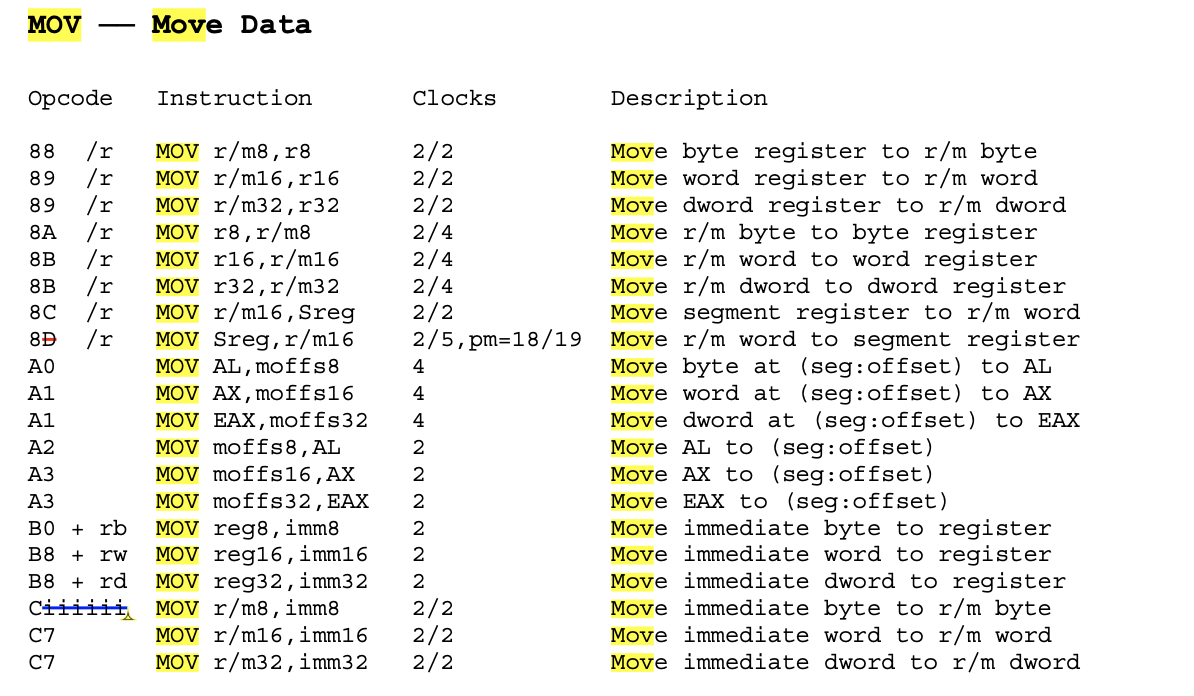
\includegraphics[scale=0.45]{fig/13.png}
                \caption{MOV格式}
            \end{figure}
        \end{enumerate}
        \item nemu/目录下的所有.c和.h和文件总共有多少行代码? 5332  $find\  -name\  "*[.h|.c]"\  -type\  f\  |\  xargs\  cat\  |\  wc\  -l$
        \item 我在PA1编写的代码427行,切到master分支,加到Makefile最后就可以了
        \item 除去空格,$find\  .\  -name\  "*[.h|.c]"|xargs\  cat|grep\  -v\  ^\$|wc\  -l$  截止pa1共4415行  
        \item 使用man 打开工程目录下的Makefile文件, 你会在CFLAGS变量中看到gcc的一些编译选项. 请解释gcc中的-Wall和-Werror有什么作用? 为什么要使用-Wall和-Werror?
        -Wall,打开gcc的所有警告,-Werror,它要求gcc将所有的警告当成错误进行处理。正如前面指导书说的,更快找到error,防止等到了fatal的时候才开始debug的手忙脚乱,比如说未定义使用函数等等。
    \end{enumerate}
}
%----------------------------------------------------------------------------- 
\section{总结}
\kt{
    30h诚不我欺,虽然写代码要不了那么久但是不停的RTFSC和为了思考题的STFW,RTFM加上写报告等等一系列确实很费时间,虽然PA是给NJU大二同学使用的,但对于我这种没有形成RTFSC体系的人,确实是一个很好的培养习惯的平台,本身的代码不难,主要是涉及的点和面比较多,这次在配置上也费了不少时间,最开始老师没有说到底32还是64位的时候(当然也是我自己没仔细看),干脆把两个都配了,虽然时间长了些,但是结果是很好的。

    总的来说,各方面都收获很多,希望下次可以再快一点。对PA理解更深一些。
}
%----------------------------------------------------------------------------- 
% \lhead{\kaishu 参考文献}
% \newpage
% \kt{
% \begin{thebibliography}{plain}  
%     \bibitem{ref1}Ray Tracing经典入门[EB/OL].https://raytracing.github.io/books/
%     \bibitem{ref2}讲稿lec2-5,8
% \end{thebibliography}
% }
\end{document}
